%<dscrpt>Nombres complexes et invariant de triangle par similitude.</dscrpt>
On se place dans un plan affine euclidien muni d'un repère orthonormé permettant d'associer une affixe complexe à chaque point du plan.
\subsection*{Partie I. Caractérisation d'un polygone régulier direct.}
Soit $n$ un entier naturel supérieur ou égal à $3$ et $A_1, A_2, \cdots , A_n$ des points deux à deux distincts dont les affixes sont $a_1,a_2,\cdots, a_n$.\newline
On note $G$ (d'affixe $g$) le centre de gravité de la famille des points $A_1, A_2, \cdots , A_n$. On rappelle que
\begin{displaymath}
 g = \frac{1}{n}(a_1 + a_2 + \cdots + a_n)
\end{displaymath}
Soit $\alpha = \frac{2\pi}{n}$ et $R$ la rotation de centre $G$ et d'angle $\alpha$.\newline
On dira que $A_1, A_2, \cdots , A_n$ est un \emph{polygone régulier direct} si et seulement si 
\begin{align*}
 A_2 = R(A_1), & & A_3 = R(A_2), & & \cdots & & A_n = R(A_{n-1}), & & A_1 = R(A_n)
\end{align*}
Au lieu de polygone régulier direct, on dira triangle équilatéral direct lorsque $n=3$ et carré direct lorsque $n=4$.
\begin{enumerate}
 \item 
Calculer sous la forme $a+ib$ avec $a$ et $b$ réels les nombres complexes suivants
\begin{displaymath}
 \frac{1+3i}{1-i},\hspace{0.5cm} \frac{3+i}{1-i}
\end{displaymath}
\item 
\begin{enumerate}
 \item Soit $Z$ (d'affixe $z$) un point du plan. Préciser l'affixe (notée $r(z)$) du point $R(Z)$.
 \item Pour $k$ entier naturel, on note $r^k = r \circ r \circ \cdots \circ r$ (composée $k$ fois). Calculer
\begin{displaymath}
 a_1 + r(a_1) + r^2(a_1) + \cdots + r^{n-1}(a_1)
\end{displaymath}
\end{enumerate}
\item 
\begin{enumerate}
 \item Montrer que $A_1, A_2, \cdots , A_n$ est un polygone régulier direct si et seulement si 
\begin{align*}
 A_2 = R(A_1), & & A_3 = R(A_2), & & \cdots & & A_n = R(A_{n-1})
\end{align*}
\item  Montrer que $A_1, A_2, \cdots , A_n$ est un polygone régulier direct si et seulement si 
\begin{align*}
 A_2 = R(A_1), & & A_3 = R(A_2), & & \cdots & & A_{n-1} = R(A_{n-2})
\end{align*}
\end{enumerate}
 \item Montrer que $A_1, A_2, A_3$ est un triangle équilatéral direct si et seulement si
\begin{displaymath}
 a_1 + ja_2 + j^2 a_3 = 0
\end{displaymath}

\item 
\begin{enumerate}
 \item Montrer que $A_1, A_2, A_3, A_4$ est un carré direct si et seulement si
\begin{displaymath}
 \left\lbrace 
\begin{aligned}
 (-1+2i)a_1 - (1+2i)a_2 + a_3 + a_4 &= 0\\
 a_1 + (-1+2i)a_2 - (1+2i)a_3 + a_4  &= 0
\end{aligned}
\right. 
\end{displaymath}
\item En combinant les lignes du système précédent, montrer que $A_1, A_2, A_3, A_4$ est un carré direct si et seulement si
\begin{displaymath}
 \left\lbrace 
\begin{aligned}
 a_1 + ia_2 &=  a_3 + ia_4 \\
 a_1 + a_3 &= a_2 + a_4
\end{aligned}
\right. 
\end{displaymath}
et interpréter géométriquement ces relations.
\end{enumerate}
 \end{enumerate}

\subsection*{Partie II. Triangles semblables.}
Soient $A$, $B$, $C$ trois points deux à deux distincts et respectivement d'affixes $a$, $b$, $c$. On note alors
\begin{displaymath}
 W(A,B,C)= \frac{ a + jb +j^2c}{ a + j^2b +jc }
\text{ lorsque } a + j^2b +jc \neq 0
\end{displaymath}
Soient $A'$, $B'$, $C'$ trois points deux à deux distincts et respectivement d'affixes $a'$, $b'$, $c'$. On dira que les triangles $(A,B,C)$ et $(A',B',C')$ sont \emph{directement semblables} si et seulement si il existe des nombres complexes $u\neq 0$ et $v$ tels que
\begin{align*}
 a' = ua + v, & & b' = ub+v, & & c' = uc +v
\end{align*}

\begin{enumerate}
\item Déterminer le réel $K$ tel que, pour tous les nombres complexes $a$, $b$, $c$,
\begin{displaymath}
 \left| a + jb +j^2c\right|^2 - \left| a + j^2b +jc\right|^2 = 
K \,\Im(a\bar{b} + b\bar{c} + c\bar{a}) 
\end{displaymath}

\item Montrer que $A$, $B$, $C$ sont alignés si et seulement si
\begin{displaymath}
 a\bar{b} + b\bar{c} + c\bar{a} \in \R
\end{displaymath}

\item
\begin{enumerate}
 \item Dans quel cas $W(A,B,C)$ est-il non défini ?
 \item Dans quel cas $W(A,B,C)$ est-il de module 1 ?
\end{enumerate}

\item 
\begin{enumerate}
 \item On suppose que $(A,B,C)$ et $(A',B',C')$ sont directement semblables. Montrer que
\begin{displaymath}
 \left\lbrace 
\begin{aligned}
 &a + j^2b +jc = a' + j^2b' +jc' =0 \\
&\text{ ou }\\
 &W(A,B,C) = W(A',B',C')
\end{aligned}
\right. 
\end{displaymath}

\item On suppose $W(A,B,C)$ et $W(A',B',C')$ définis et égaux. Montrer que $(A,B,C)$ et $(A',B',C')$ sont directement semblables.
\end{enumerate}

\item On suppose que $W(A,B,C)$ est défini et que les points $A'$, $B'$, $C'$ ont respectivement pour affixe $\bar{a}$, $\bar{b}$, $\bar{c}$. Dans quel cas $W(A',B',C')$ est-il défini ? Exprimer le alors en fonction de $W(A,B,C)$.
\end{enumerate}

\subsection*{Partie III. Construction.}
\begin{figure}[h!t]
 \centering
 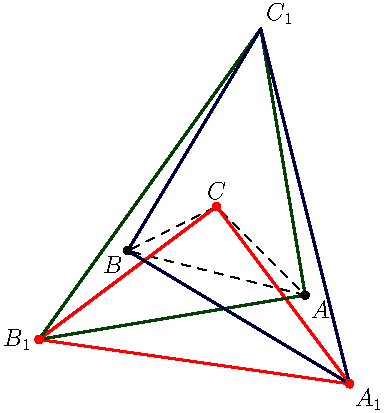
\includegraphics{./Ecomp12_1.pdf}
 % Ecomp12_1.pdf: 76x227 pixel, 72dpi, 2.68x8.01 cm, bb=0 0 76 227
 \caption{Triangles formés avec $A_1$, $B_1$, $C_1$}
 \label{fig:Ecomp12_1}
\end{figure}
Soient $A$, $B$, $C$ trois points d'affixes $a$, $b$, $c$. On les suppose deux à deux distincts et non alignés. On définit les points $A_1$, $B_1$, $C_1$ d'affixes $a_1$, $b_1$, $c_1$ par les relations
\begin{align*}
 a_1 = a + i(b-c), & & b_1 = b + i(c-a), & & c_1 = c + i(a-b)
\end{align*}
\begin{enumerate}
 \item 
\begin{enumerate}
 \item Les points $A$, $B$, $C$ étant donnés, comment peut-on construire $A_1$, $B_1$, $C_1$ ?
 \item Montrer que les triangles $(A, B, C)$ et $(A_1, B_1, C_1)$ ont le même centre de gravité.
 \item Montrer que les triangles $(A_1,B_1,C)$, $(B_1,C_1,A)$, $(C_1,A_1,B)$ sont rectangles et isocèles.
\end{enumerate}

\begin{figure}[h!t]
 \centering
 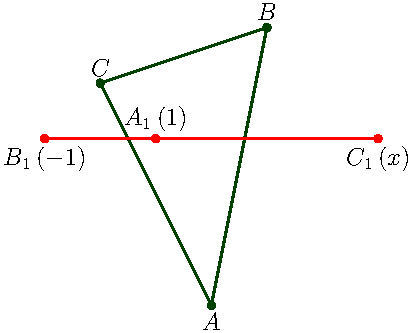
\includegraphics{./Ecomp12_2.pdf}
 \caption{$A_1$, $B_1$, $C_1$ alignés sur l'axe réel}
 \label{fig:Ecomp12_2}
\end{figure}

\item On admet (fig \ref{fig:Ecomp12_2}) qu'il existe des points $A$, $B$, $C$ tels que les affixes de $A_1$, $B_1$, $C_1$ soient respectivement $1$, $-1$ et $x\in\R$.
\begin{enumerate}
\item Exprimer $a$, $b$, $c$ en fonction de $x$.
\item Quels sont les ensembles décrits par $A$, $B$, $C$ lorsque $x$ varie dans $\R$ ?
\end{enumerate}

\item On cherche à déterminer si les triangles $(A, B, C)$ et $(A_1, B_1, C_1)$ peuvent être directement semblables.
\begin{enumerate}
 \item Mettre sous la forme $u+iv$ avec $u$ et $v$ réels les nombres complexes suivants
\begin{align*}
 1-ij+ij^2, & & i + j -ij^2, & & -i+ij+j^2
\end{align*}
 \item Exprimer $a_1+jb_1+j^2c_1$ en fonction de $a+jb+j^2c$.
 \item Exprimer $a_1+j^2b_1+jc_1$ en fonction de $a+j^2b+jc$.
 \item Montrer que si $(A, B, C)$ et $(A_1, B_1, C_1)$ sont directement semblables alors $(A,B,C)$ est équilatéral.
 \item Montrer que si $(A,B,C)$ est équilatéral alors $(A, B, C)$ et $(A_1, B_1, C_1)$ sont directement semblables et préciser le centre, le rapport et l'angle de la similutude.
\end{enumerate}

\end{enumerate}
